% mnras_template.tex 
%
% LaTeX template for creating an MNRAS paper
%
% v3.0 released 14 May 2015
% (version numbers match those of mnras.cls)
%
% Copyright (C) Royal Astronomical Society 2015
% Authors:
% Keith T. Smith (Royal Astronomical Society)

% Change log
%
% v3.0 May 2015
%    Renamed to match the new package name
%    Version number matches mnras.cls
%    A few minor tweaks to wording
% v1.0 September 2013
%    Beta testing only - never publicly released
%    First version: a simple (ish) template for creating an MNRAS paper

%%%%%%%%%%%%%%%%%%%%%%%%%%%%%%%%%%%%%%%%%%%%%%%%%%
% Basic setup. Most papers should leave these options alone.
\documentclass[fleqn,usenatbib]{mnras}

% MNRAS is set in Times font. If you don't have this installed (most LaTeX
% installations will be fine) or prefer the old Computer Modern fonts, comment
% out the following line
\usepackage{newtxtext,newtxmath}
% Depending on your LaTeX fonts installation, you might get better results with one of these:
%\usepackage{mathptmx}
%\usepackage{txfonts}

% Use vector fonts, so it zooms properly in on-screen viewing software
% Don't change these lines unless you know what you are doing
\usepackage[T1]{fontenc}
\usepackage{ae,aecompl}


%%%%% AUTHORS - PLACE YOUR OWN PACKAGES HERE %%%%%

% Only include extra packages if you really need them. Common packages are:
\usepackage{graphicx}	% Including figure files
\usepackage{amsmath}	% Advanced maths commands
\usepackage{amssymb}	% Extra maths symbols
\usepackage{color}
\usepackage{aas_macros}
\usepackage{hyperref,breakurl}
\usepackage[usenames,dvipsnames]{xcolor}
\usepackage{dcolumn}
\usepackage{bm}
\usepackage{hyperref}
\usepackage{array}
\usepackage{dcolumn}
\usepackage{subfig}
\usepackage{amsmath,amssymb,latexsym,times}

\usepackage{todonotes}

\graphicspath{{figures/}}


\newcommand{\verify}[1]{\textcolor{red}{\textbf{{#1}}}}

\newcommand\assign[1]{\todo[color=RoyalPurple!40, inline, size=\small]{Contributing: #1}}
\newcommand\troxel[1]{\todo[color=cyan!40, inline, size=\small]{Troxel: #1}}
\newcommand\zhou[1]{\todo[color=magenta!40, inline, size=\small]{Zhou: #1}}
\newcommand\alex[1]{\todo[color=LimeGreen, inline, size=\small]{Alex: #1}}
\newcommand\ct[1]{\textcolor{red}{(#1)}}


%%%%%%%%%%%%%%%%%%%%%%%%%%%%%%%%%%%%%%%%%%%%%%%%%%

%%%%% AUTHORS - PLACE YOUR OWN COMMANDS HERE %%%%%

% Please keep new commands to a minimum, and use \newcommand not \def to avoid
% overwriting existing commands. Example:
%\newcommand{\pcm}{\,cm$^{-2}$}	% per cm-squared

%%%%%%%%%%%%%%%%%%%%%%%%%%%%%%%%%%%%%%%%%%%%%%%%%%

%%%%%%%%%%%%%%%%%%% TITLE PAGE %%%%%%%%%%%%%%%%%%%

% Title of the paper, and the short title which is used in the headers.
% Keep the title short and informative.
\title[Intrinsic alignment in DES Y1 redMaPPer clusters]{Redshift evolution of the intrinsic alignment of galaxies in DES Y1 RedMaPPer galaxy clusters}

% The list of authors, and the short list which is used in the headers.
% If you need two or more lines of authors, add an extra line using \newauthor
\author[K. T. Smith et al.]{
(no order yet) M.~A. Troxel,$^{1}$\thanks{E-mail: michael.troxel@duke.edu (MAT)}
Conghao Zhou,$^{1}$
Alexander Tong$^{1}$
and othres$^{1}$
\\
% List of institutions
$^{1}$Department of Physics, Duke University, Durham, NC 27708, USA\\
}

% These dates will be filled out by the publisher
\date{Accepted XXX. Received YYY; in original form ZZZ}

% Enter the current year, for the copyright statements etc.
\pubyear{2019}

\begin{document}
\label{firstpage}
\pagerange{\pageref{firstpage}--\pageref{lastpage}}
\maketitle

\begin{abstract}
Clusters of galaxies are an interesting cosmological probe, sensitive to the most significant and nonlinear peaks in the cosmic density field. The weak gravitational lensing of background galaxies by foreground clusters can allow us to infer the mass of galaxy clusters. However, galaxies associated with the strong, local tidal field of the cluster can also be intrinsically aligned relative to the tidal gradient, potentially contaminating any cosmology derived from the lensing signal. We measure this intrinsic alignment in Dark Energy Survey Year 1 RedMaPPer clusters and find a significant detection of mean radial alignment of luminous red galaxies within clusters between redshift 0.X and 0.X at XXX$\sigma$. We are able to place constraints on the redshift evolution of this signal, finding a stronger alignment at low/high redshift using multiple metrics.
\end{abstract}

\begin{keywords}
cosmology: observations -- gravitational lensing: weak -- galaxies: clusters: general 
\end{keywords}

%%%%%%%%%%%%%%%%%%%%%%%%%%%%%%%%%%%%%%%%%%%%%%%%%%

%%%%%%%%%%%%%%%%% BODY OF PAPER %%%%%%%%%%%%%%%%%%



% This is a simple template for authors to write new MNRAS papers.
% See \texttt{mnras\_sample.tex} for a more complex example, and \texttt{mnras\_guide.tex}
% for a full user guide.

% All papers should start with an Introduction section, which sets the work
% in context, cites relevant earlier studies in the field by \citet{Others2013},
% and describes the problem the authors aim to solve \citep[e.g.][]{Author2012}.


\section{Introduction}
In 1919, Arthur Eddington and Frank Dyson verified the theory of general relativity by observing the deflection of the light by the sun, which is aptly named gravitational lensing. 100 years after the Eddington experiment, gravitational lensing, especially in the weak regime, has become one of the most powerful probes in modern cosmology surveys. Weak lensing probes including galaxy-galaxy lensing, cluster lensing, and cosmic shear, combined with other types of probes, can constrain cosmological parameters effectively and thus reveal the growth history of the universe. The recent growth of data volume from Stage III surveys such as DES, KiDS, and HSC \ct{Hildebrandt, Amon, Aihara} \verify{is this three papers?} has significantly lowered the statistical errors in the lensing signal. And thus lowering the systematic errors are critical for extracting weak lensing signals from existing and future survey. One source of systematic error in weak lensing is from the correlated intrinsic alignment signals that contaminate shear correlations. The intrinsic alignment of galaxies are caused by a variety of physical processes during the structure formation. The intrinsic alignment of galaxies acts as a nuisance signal to the lensing signal measurement and can strongly bias results we get from it. The constraint of the equation of dark energy can be biased by 50\% or more by intrinsic alignment. Similarly, the amplitude of matter fluctuations can be biased by 30\%. Isolating intrinsic alignment signal not only improve the result we get from lensing surveys but also provides insights to the evolution of galaxies.\ct{Troxel}

In the framework of $\Lambda$CDM cosmology, one of the most natural places for the intrinsic alignment between galaxies to emerge is within clusters of galaxies \ct{White, Rees}. 




\section{Dark Energy Survey Year 1 Data}
The Dark Energy Survey is a six-year survey covering 5000 square degrees of the southern sky using the Dark Energy Camera \cite{decam} mounted on the Blanco 4m telescope in Cerro Tololo, Chile. Observations use five broadband filters $g, r, i, z , Y$. The first year of DES observations lasted from August 2013 to February 2014 and covers ~40\% of the total DES footprint \cite{y1gold}. We use data based on several value-added catalogs built from the Y1 data: 1) the Y1A1 GOLD catalog, a high quality photometric data set; 2) the red-sequence Matched-filter Probabalistic Percolation (redMaPPer) cluster and member catalogs; 3) the \textsc{metacalibration} and \textsc{im3shape} shape catalogs. 

\subsection{GOLD Catalog}
\label{sec:y1a1gold}
The Y1A1 GOLD data set \cite{} is a high quality photometric catalog that contains multi-epoch, multi-object photometric model parameters and other ancillary information. The objects in this catalog are selected from the initial Y1A1 coadd detection catalog, which is processed by the DESDM image processing pipeline \cite{2011arXiv1109.6741S,2008SPIE.7016E..0LM}. The Y1A1 GOLD catalog restricts the footprint of the catalog to regions with at least one image of sufficient science quality in each filter. Several bad region mask including unphysical colors, the Large Magellanic Cloud, globular clusters, and bright stars are masked. The final Y1A1 GOLD footprint covers ~1800 deg$^2$ with an average of three to four single-epoch image per band. The photometric accuracy is \(\lesssim 2 \%\) over the survey area. A comparison with the deeper catalog of the Canada-France-Hawaii Telescope Lensing Survey shows that the Y1A1 GOLD catalog is $>$ 99\% complete in $g,r,i,z$ bands for magnitudes brighter than 21.5. There are approx. 137 million objects in the final Y1A1 GOLD catalog.

\subsection{RedMaPPer cluster catalog}
\label{sec:redmapper} % used for referring to this section from elsewhere

The red-sequence Matched-filter Probabalistic Percolation (redMaPPer) photometric cluster finding algorithm is optimized for deep-field photometric cosmology surveys \cite{2014ApJ...785..104R} and produces a cluster catalog identifying overdensities of red-sequence galaxies with a probabalistic assignment of these red-sequence galaxies as central/satellite members. This alogorithm has been validated using X-ray and Sunyaev-Zel'dovich (SZ) observations \cite{2015MNRAS.453...38R,2015MNRAS.454.2305S,2016MNRAS.461.1431R,2014A&A...571A..87S}, and updates to the method are described in \cite{2016MNRAS.461.1431R,2016ApJS..224....1R,2019MNRAS.482.1352M}. We briefly describe the algorithm and resulting cluster catalog below.

To identify clusters, the redmapper algorithm counts the excess number of red-sequence galaxies, called the richness ($\lambda$), within a radius $R_\lambda = 1.0\ \hinv\ \Mpc (\lambda/100)^{0.2}$ that are brighter than some luminosity threshold $L_{\mathrm{min}}(z)$. A locally volume-limited version of the catalog is also produced, which imposes a maximum redshift on clusters such that galaxies above $L_{\mathrm{min}}(z)$ can be detected at 10$\sigma$. An associated redshift-dependent random catalog for both cluster catalogs is produced using a survey mask constructed to require that a cluster at redshift $z$ at each point in the mask be masked by at most 20\% by the associated galaxy footprint mask.

The algorithm centers each cluster on the most likely central galaxy, based on an iterativley trained filter relying on galaxy brightneess, cluster richness, and local density. to determine the central candidate probability. Each red-sequence cluster member is also assigned an associated membership probability, which we weight all measurements by. Additional information about the quality of photometric redshifts of the clusters and cluster members can be found in \cite{2019MNRAS.482.1352M,wthetapaper}, but over most of the redshift range used in this paper cluster redshifts are unbiased at the level of $|\Delta z| \leq 0.003$ with a median photometric redshift scatter of $\sigma_z/(1+z)\approx 0.006$. For red-sequence cluster members, this is... XXX

In this work, we use a total of XXX clusters from the DES Y1 redMaPPer catalog (XXX in the volume-limited catalog). Within these clusters, there are an effective number of XXX (XXX) cluster members (central/satellite galaxies). We include clusters outside the range used for cosmology in \cite{2020arXiv200211124D} in order to increase our statistical power, but use the same $\lambda>20$ selection on richness, since inference of the halo shape based on the distribution of satellite galaxies is increasingly difficult as the number of satellite galaxies decreases. The redshift distribution of the final sample of clusters is shown in Fig. \ref{fig:zdist}.



\begin{figure}
\begin{center}
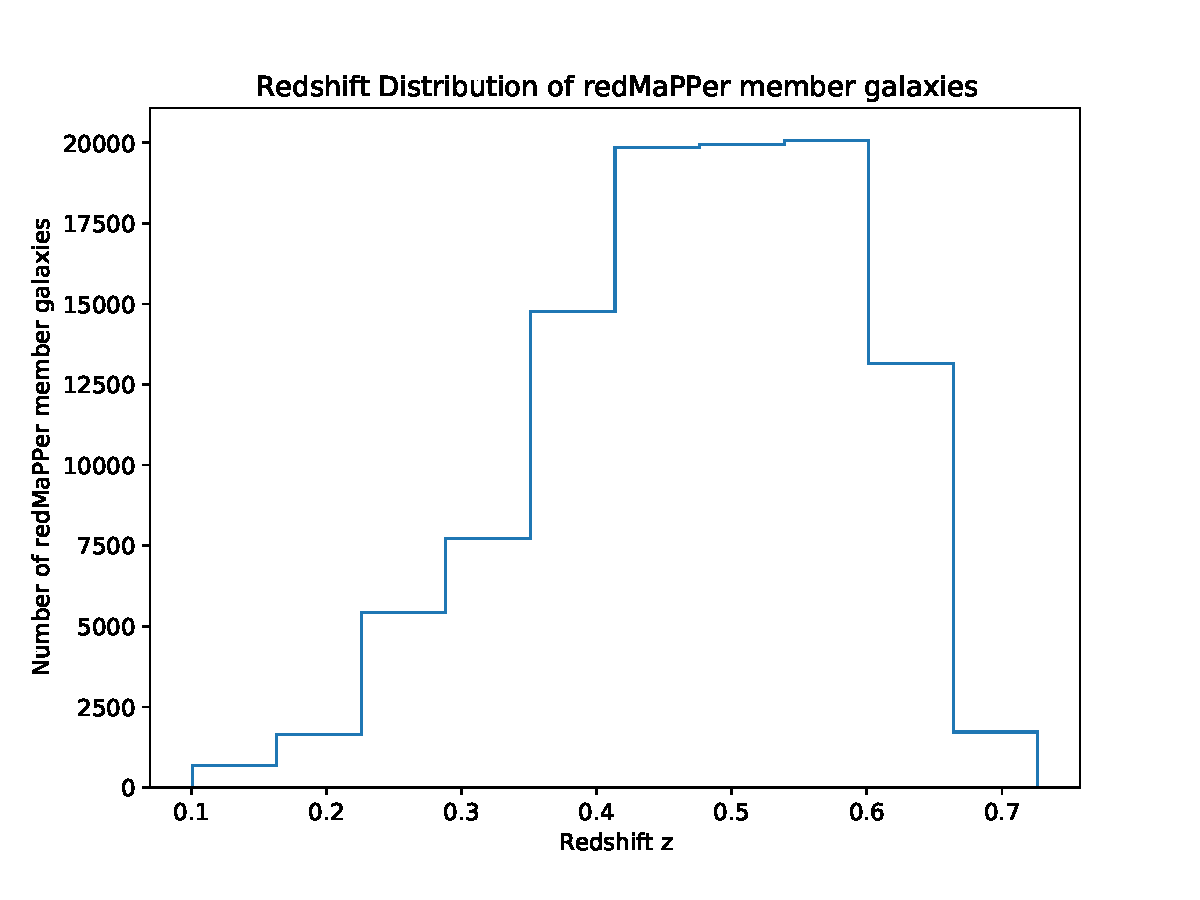
\includegraphics[width=\columnwidth]{z_hist.pdf}
\end{center}
\caption[]{The redshift distribution of redMaPPer clusters used in this work.
\label{fig:zdist}}
\end{figure}

\subsection{Shape Catalogs}

We use a fiducial shape catalog that is calibrated with the \textsc{metacalibration} method, which uses available imaging data directly without the need for significant prior information as a function of galaxy properties or expensive calibration from image simulations \cite{HuffMandelbaum2017,SheldonHuff2017}. The \textsc{metacalibration} implementation used in DES was described in detail in \cite{shearcat}. Limitations in the DES Y1 implementation of \textsc{metacalibration} lead to a residual mean multiplicative shear bias estimate of $m = 0.012 \pm 0.013$, which is due primarily to the effects of neighboring light on the shear recover. This mean correction is applied to the the measurements in this work. 

\textsc{metacalibration} also allows us to account for sample selection bias effects, as described in \cite{shearcat,shearcorr}, which we also include. However, we match the shape catalog to the redMaPPer central/satellite member catalog, which introduces an additional selection that we cannot incorporate in the selection bias correction. In future work, we plan to explore the impact of this selection by running the redMaPPer selection algorithm on the photometry produced in the \textsc{metacalibration} process similar to how we incorporate redshift selection biases in, e.g., \cite{shearcorr}. At the current precision of the measurements in this paper, however, we expect this additional correction to be safely negligible.

The \textsc{metacalibration} catalog yields a total of 35 million objects, XXX of which are used in the selection for the current analysis matched to the redMaPPer central/satellite members. We are able to match a \textsc{metacalibration} shape measurement to XXX\% of redMaPPer members. We also compare measurements using the \textsc{im3shape} shape catalog \cite{shearcat,2013MNRAS.434.1604Z}, which utilizes a simulation-based calibration and only has secure shape measurements for XXX\% of redMaPPer members.

% Example table
% \begin{table}
% 	\centering
% 	\caption{This is an example table. Captions appear above each table.
% 	Remember to define the quantities, symbols and units used.}
% 	\label{tab:example_table}
% 	\begin{tabular}{lccr} % four columns, alignment for each
% 		\hline
% 		A & B & C & D\\
% 		\hline
% 		1 & 2 & 3 & 4\\
% 		2 & 4 & 6 & 8\\
% 		3 & 5 & 7 & 9\\
% 		\hline
% 	\end{tabular}
% \end{table}


\begin{figure}
\begin{center}
%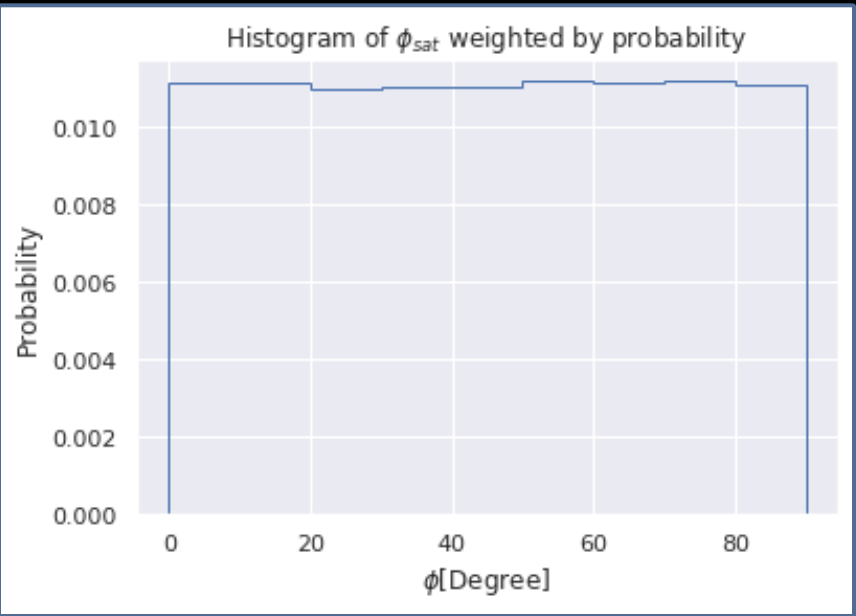
\includegraphics[width=\columnwidth]{phisat.png}
\end{center}
\caption[]{Figure summarizing angles used in sec \ref{methods}
\label{fig:phisat}}
\end{figure}

\section{Methods to infer the intrinsic alignment of galaxies in clusters}\label{methods}

The intrinsic alignment of galaxies in the (quasi-)linear regime is typically expressed via perturbation theory as a function of the underlying tidal field. Most cosmological studies have used a linear alignment model \cite{} that uses the first order expansion of the intrinsic shear $\gamma^I$ (shown here up to second order) in the linear density field:
\begin{equation}
    \gamma^I(\bm{x}) = C_1 s_{ij}+C_2\left(s_{ik}s_{kj}-\frac{1}{3}\delta_{ij}s^2\right)+C_{1\delta}(\delta s_{ij})+C_t t_{ij}+\cdots,
\end{equation}
where each field is evaluated at $\bm{x}$ and summation occurs over repeated indices. The $C_i$ parameters are then the analog to galaxy bias parameters in perturbation theory, and $\delta_{ij}$ is the Kronecker delta, $\delta$ is the density field, $s_{ij}(\bm{k})\equiv\hat{S}_{ij}[\delta(k)]$ is the normalized Fourier-space tidal tensor, $S^2(\bm{k})$ is the tidal tensor squared, and the tensor $t_{ij}=\hat{S}_{ij}[\theta-\delta]$ involves the velocity shear. From this, one can build up all standard components of commonly used intrinsic alignment models up to second order in the density field, as described in detail in \cite{blazek}.

When modelling the intrinsic alignment of galaxies in strongly nonlinear environments like galaxy clusters, where perturbative models will break down, it has been proposed to use a `1-halo' model in analogy to the halo model for the matter power spectrum to describe alignments internal to a single cluster halo. This has been discussed by \cite{SB10, 2003.02700}, which outline approaches for building such a model, including tests on simulations. Previous attempts to directly measure such a signal, e.g. within galaxy clusters, have had mixed results both in simulations and data. These fall into two categories: 1) the alignment of the cluster shape with the tidal field \cite{} and 2) the alignment of satellite galaxies \cite{}, using the cluster center as a proxy for the local tidal field. 

Better measurements of the 1-halo intrinsic alignment signal are necessary to inform and constrain such a beyond-perturbative model, however, which is the goal of this paper. While most measurement attempts have focused on objects with spectroscopic redshifts, which suffer from limited data volumes, We present several complementary measurements of these alignments using a fully photometric galaxy cluster and satellite catalog that selects red-sequence galaxies and spans over 1000 deg$^2$ to redshift \verify{0.8}.

\subsection{Orientation of the satellite galaxy distribution}\label{pamethod}

We quantify the strength of the central galaxy alignment relative to the orientation of the cluster satellite distribution as a proxy for the dark matter halo in two ways, which were also used in SDSS for redMaPPer clusters by \cite{Huang_2016}. First, the position angle difference between the central galaxy and its host cluster $\Delta \eta$, and second, the central galaxy alignment angle for each central-satellite pair $\theta _{cen}$. They are both defined to lie in the range $[0 \degree , 90 \degree]$, with values closer to $0 \degree$ indicating stronger central galaxy alignment.

Measuring $\Delta \eta$ requires an approximation of the overall cluster shape from the distribution of satellite galaxies. We use 2 different methods to determine the ellipticity and orientation of the cluster in order to measure $\Delta \eta$.

\subsubsection{Method 1: Second moments}

We follow the method used by \citet{Huang_2016} to calculate the cluster ellipticity and position angle. We use all satellite galaxies with $p_{\mathrm{mem}} \geq 0.2$ in order to reasonably trace the shape of the cluster. We first calculate the reduced second moments of the positions of all remaining satellite galaxies in the cluster:
\begin{equation}
    M_{xx} \equiv \frac{\sum_i p_{i,\mathrm{mem}} \frac{x_i^2}{r_i^2}}{\sum_i p_{i,\mathrm{mem}}}, M_{xy} \equiv \frac{\sum_i p_{i,\mathrm{mem}} \frac{x_i y_i}{r_i^2}}{\sum_i p_{i,\mathrm{mem}}}, M_{yy} \equiv \frac{\sum_i p_{i,\mathrm{mem}} \frac{y_i^2}{r_i^2}}{\sum_i p_{i,\mathrm{mem}}}
\end{equation}
\verify{what is r - cartesian distance}
where $x_i$ and $y_i$ are the distances of satellite galaxy $i$ from the central galaxy in RA and Dec, respectively. We then use the Stokes parameters to define the cluster shape as follows:
\begin{equation}
    (Q, U) = \frac{1-b^2/a^2}{1+b^2/a^2} (\cos 2\beta, \sin 2\beta) = (M_{xx} - M_{yy}, 2M_{xy})
\end{equation}
where $b/a$ is the cluster minor-to-major axis ratio and $\beta$ is the cluster position angle (PA).

\subsubsection{Method 2: Quadrant grid}

Our second method for measuring cluster shapes is based on the assumption that satellite projections are distributed isotropically within a 2D ellipse around the central galaxy. We place a set of orthogonal axes on the central galaxy in the plane of the sky, rotated at different angles $\theta$ relative to the central galaxy position angle, and count the satellites in each quadrant ($q$).

We define the count difference in cross-pair quadrants as $m = q_1 + q_3 - q_2 - q_4$, which we can model as a function of $\theta$. The assumption of 2D ellipse leads to the following expression for $m(\theta)$:
% \begin{equation}
%     m (\theta) = \frac{N}{2\pi} (\tan^{-1} (\frac{\tan (\theta - \beta + \pi/2)}{r}) + 
%                                  \tan^{-1} (\frac{\tan (\theta - \beta - \pi/2)}{r}) \\
%                                  -\tan^{-1} (\frac{\tan (\theta - \beta)}{r}))
% \end{equation}
\begin{equation}
m(\theta) = \frac{N}{2\pi}\left[ \arctan\left(\frac{\tan(\beta - \theta)}{r}\right) + 2 \arctan\left(\frac{\cot(\beta - \theta)}{r}\right) \right]
\end{equation}
where $N$ is the number of satellites in the cluster, $\beta$ is the cluster position angle, and $r$ is the minor-to-major axis ratio $b/a$. We fit this model to the count difference data as a function of $\theta$ and find the best-fit parameters $\beta$ and $r$, which together completely describe the shape of the cluster. An example cluster with the best-fit shape model over-plotted is shown in Fig. \ref{fig:cluster}.

\begin{figure}
\begin{center}
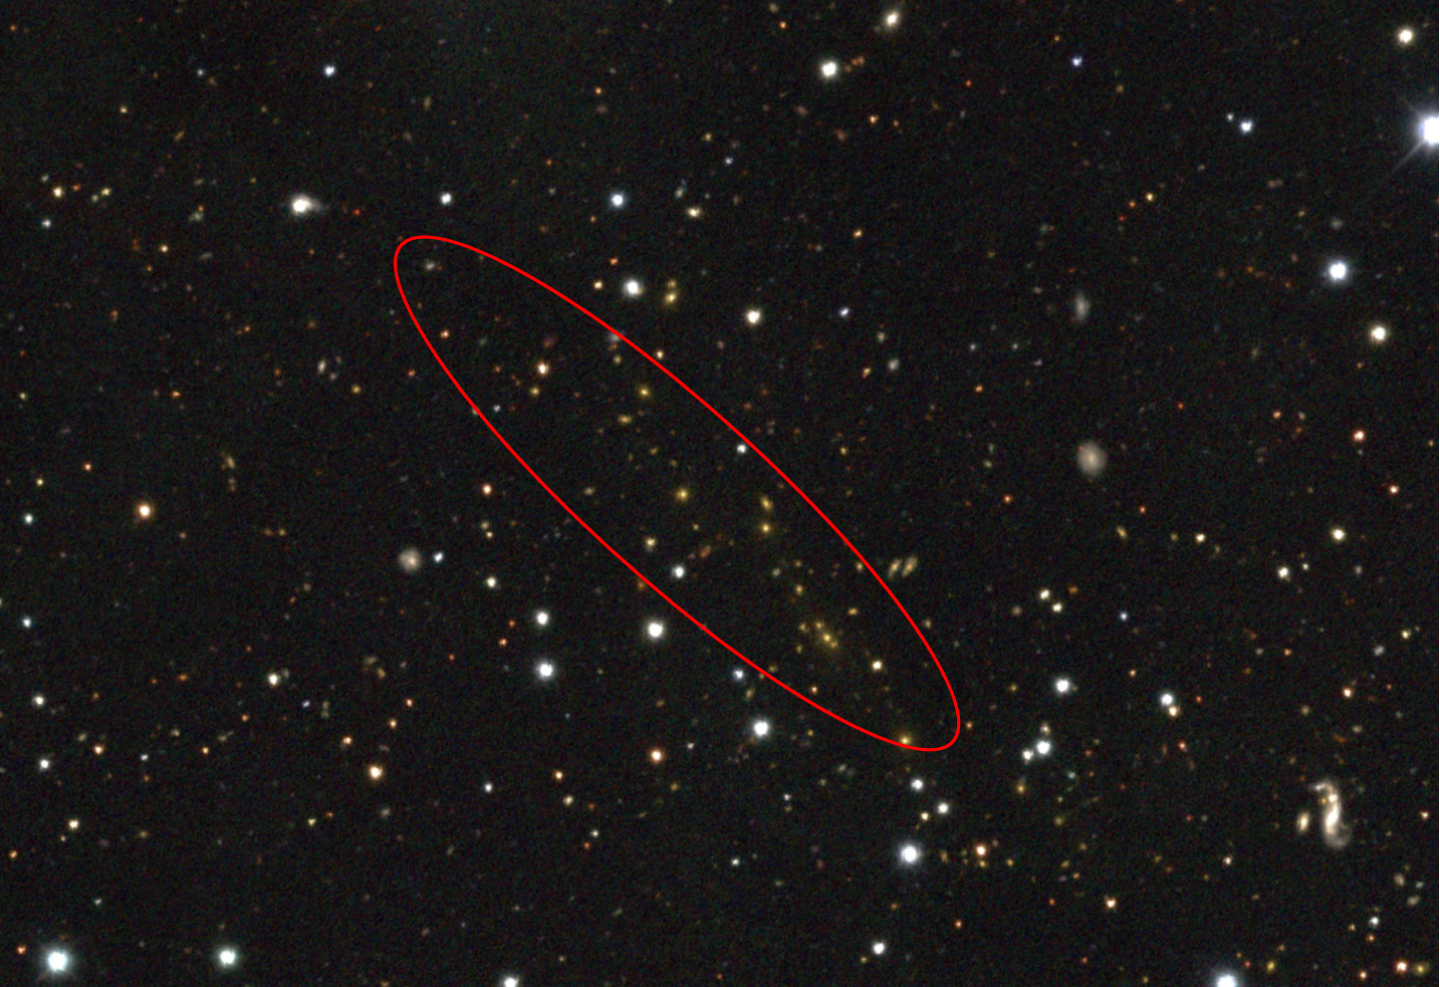
\includegraphics[width=\columnwidth]{cluster_example.png}
\end{center}
\caption[]{An example cluster at $z=0.41$ with its shape fit by Method 2 over-plotted. This cluster was found to have $e=0.73$, with a position angle 48\textdegree~east-of-north and redMaPPer radius 0.746 Mpc. 
\label{fig:cluster}}
\end{figure}


\begin{figure}
\begin{center}
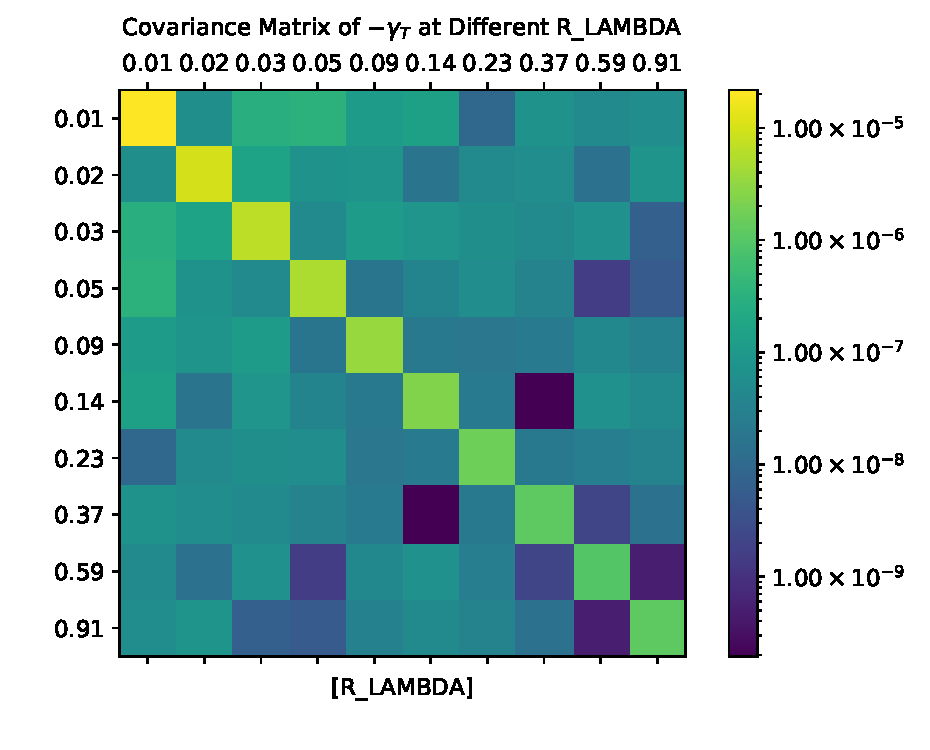
\includegraphics[width=\columnwidth]{cov_lognorm.pdf}
\end{center}
\caption[]{The jackknife covariance matrix for the full-sample $gamma_r(R)$ measurement, discussed in Secs. \ref{methodradial} \& \ref{radial}. As expected for shot or shape noise, the covariance is strongly diagonal.
\label{fig:cov}}
\end{figure}

\subsection{Radial alignment of satellite galaxies with the cluster center}\label{methodradial}

The tendency of satellite galaxies to align radially with their major axis pointed toward the central galaxy is another measure of the influence of the cluster's tidal field on the orientation of galaxies within its dark matter halo. While the mechanism for this alignment, e.g., whether it is achieved over time or during the galaxies formation, is not clear, we can place empirical constraints on this alignment at the time we observe the cluster. 

One way to parameterize this alignment is similar to the observables described in the preceding section, which we will label $\phi_{\mathrm{sat}}$ following \cite{Huang_2017}. This is the angle between the position angle of the satellite galaxy and the line connecting it to the central galaxy. Another standard method is calculating the mean radial shape $\gamma_r(R)$ 
\begin{equation}
\gamma_r(R) = -\frac{\sum_{i} p_{i,\mathrm{mem}} e_{i,+}}{\sum_{i} p_{i,\mathrm{mem}}}
\end{equation}
via the two-point correlation function of the central galaxy positions with the ellipticity of the satellite galaxies. $R$ is the projected distance separation of the satellite from the central galaxy of the cluster, $i$ is some satellite galaxy in some cluster, and $e_{+}$ is the component of the ellipticity projected along a basis coinciding with the line connecting the satellite galaxy to the central galaxy of the cluster, where positive is taken to be the radial direction.

\begin{figure}
\begin{center}
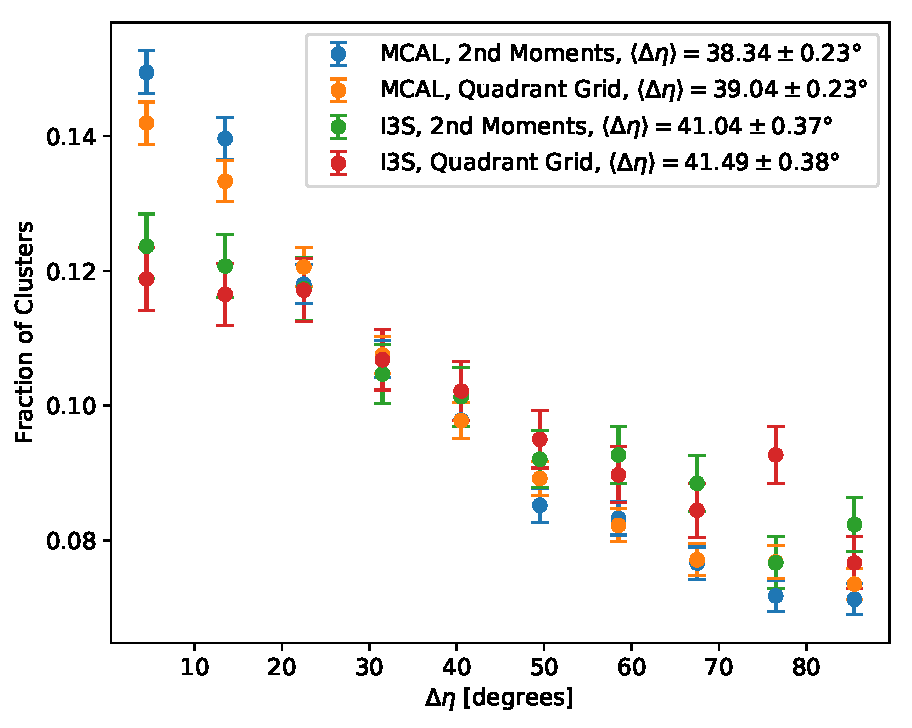
\includegraphics[width=\columnwidth]{padif_methods_catalogs.pdf}
\end{center}
\caption[]{The distribution of position angle differences ($\Delta \eta$) between the BCG major axis and that of the satellite galaxy distribution for the DES Y1 galaxy clusters. The inferred PA is derived from two different shape catalogs, metacalibration (MCAL) and im3shape (I3S), as well as two different methods for inferring the major axis, as described in Sec. \ref{pamethod}. The results are generally consistent, though the two shape catalogs in particular lead to disagreement in the number of clusters with extreme $\Delta \eta$. 
\label{fig:padiff1}}
\end{figure}



\subsection{Estimating the covariance of measurements}

Lacking a robust a priori theoretical model for what the measured signals should be, we cannot construct a theoretical covariance framework. Instead we rely on a jackknife covariance estimate, iteratively removing each cluster from the sample. The covariance is then given by
\begin{equation}
C_{\xi}(x) = \frac{N-1}{N}\sum_{i=1}^N (\xi_i-\bar{\xi})^2,
\end{equation}
where $N$ is the number of clusters, $i$ is the cluster number, and $\bar{\xi}=\sum_i \xi_i/N$, for some estimator $\xi$. The covariances are expected to be dominated by shot or shape noise, given the small sample sizes, so we expect the jackknife approach to be sufficiently accurate. In particular, the measurement of $\gamma_r$ in Sec. \ref{radial}, which is the most substantial result in this work, is non-zero only for very small separations, where shape noise dominates the correlation function. The covariance matrix for $\gamma_r$ is shown in Fig. \ref{fig:cov}.

\section{Measured alignment in DES clusters}

\subsection{Alignment of central galaxy with satellite galaxy distribution}\label{align1}

\begin{figure}
\begin{center}
% 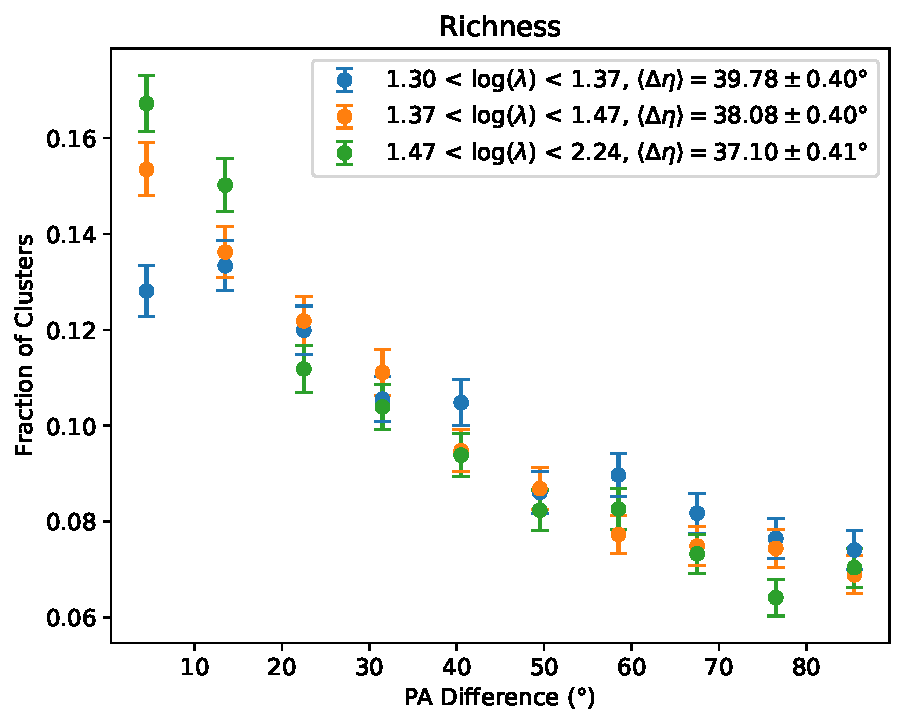
\includegraphics[width=0.8\columnwidth]{padif_2mom_lambda.pdf}
% 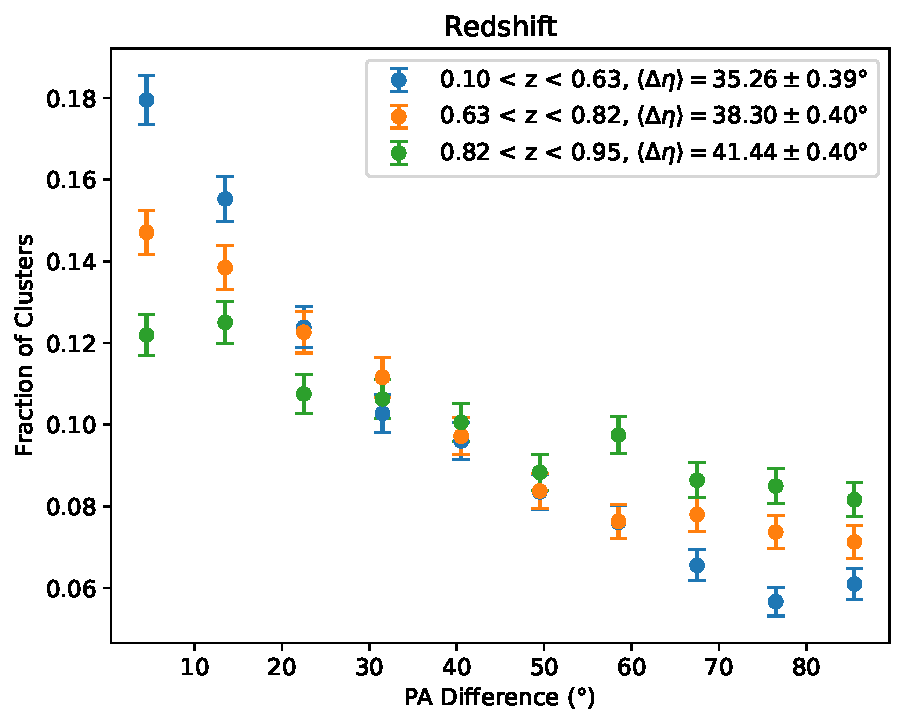
\includegraphics[width=0.8\columnwidth]{padif_2mom_redshift.pdf}
% 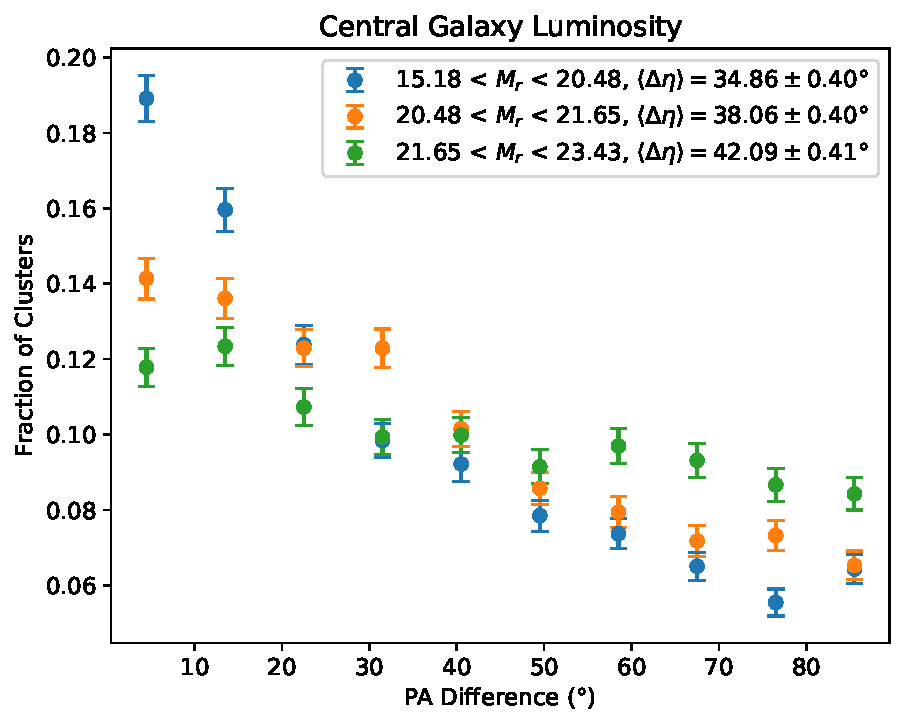
\includegraphics[width=0.8\columnwidth]{padif_2mom_Mr.pdf}
% 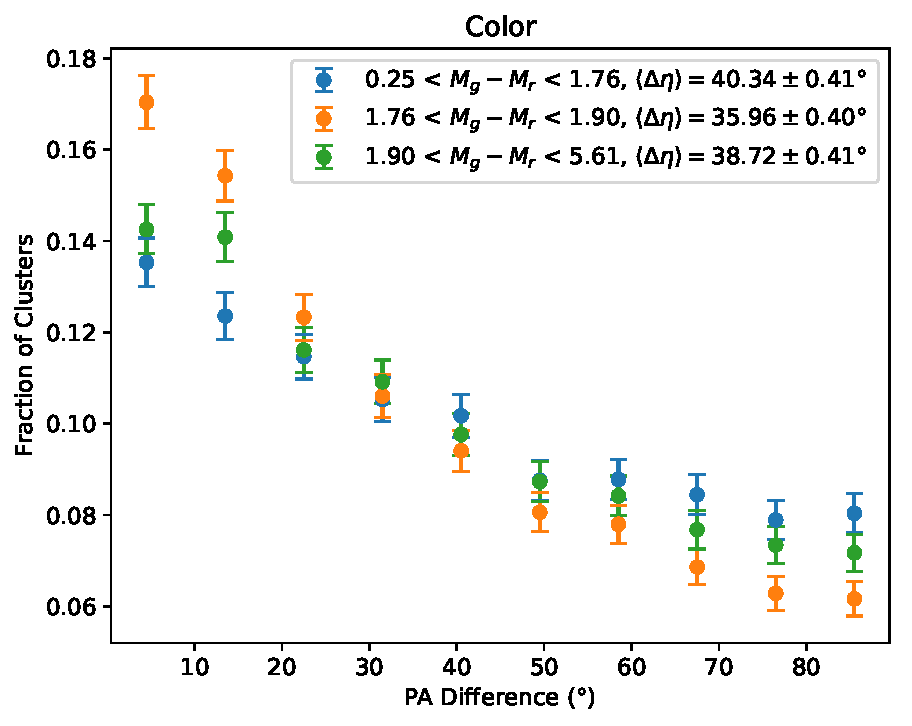
\includegraphics[width=0.8\columnwidth]{padif_2mom_color.pdf}
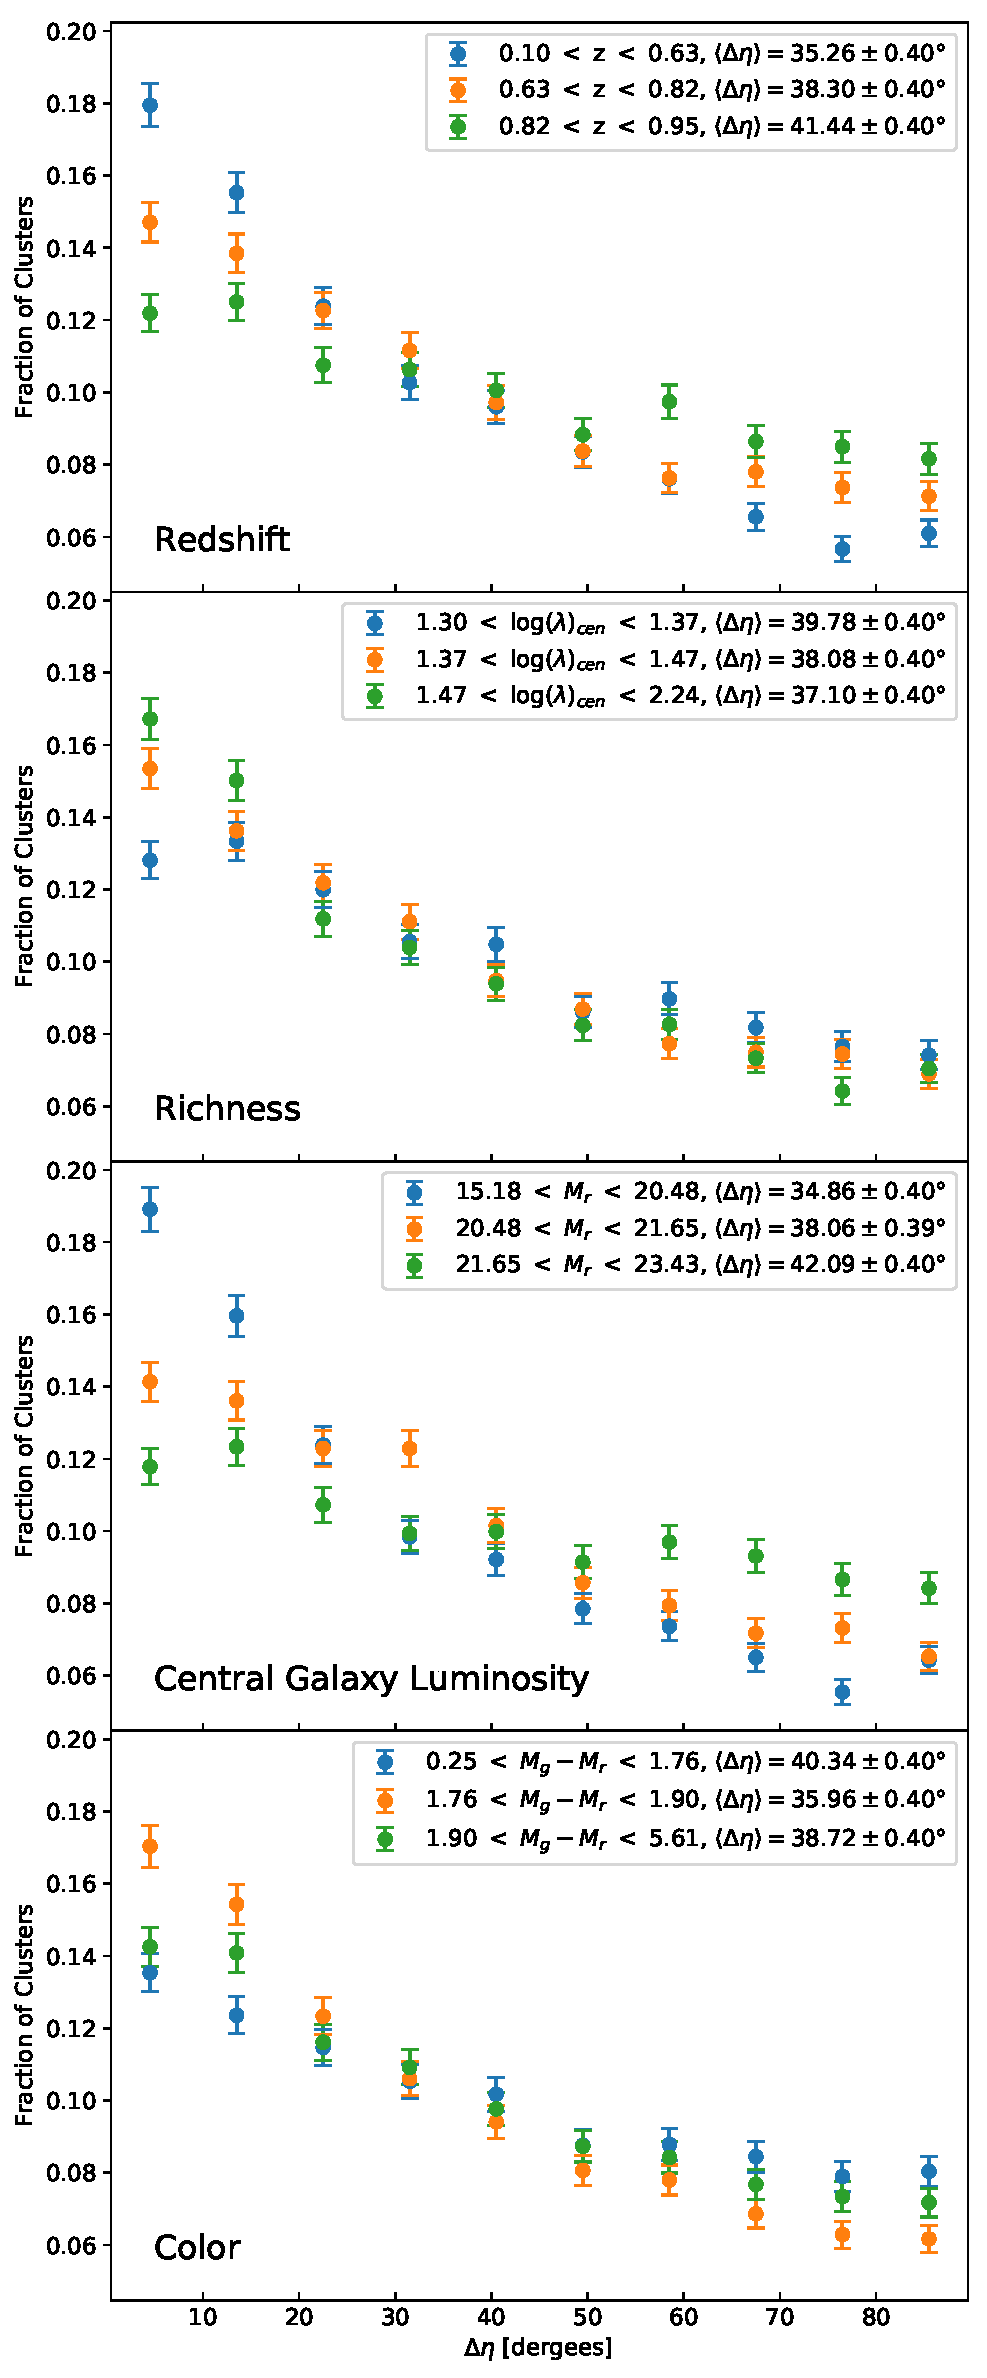
\includegraphics[width=\columnwidth]{padif_2mom_stacked.pdf}
\end{center}
\caption{The position angle difference, as described in Fig. \ref{fig:padiff1}, with clusters split into tertiles of richness, redshift, and central galaxy $r$-band absolute magnitude $M_r$ and $g$-$r$ color. We find clear trends in stronger alignment of the central galaxy with the cluster shape when going to higher richness and central galaxy brightness, which are both a proxy for cluster mass. We also find a trend of stronger alignment at lower redshift. \verify{Mr is abs mag}
\label{fig:padiff2}}
\end{figure}

We first compare measurements of the position angle difference $\Delta \eta$, weighted by the probability of satellite galaxies being a cluster member $p_{\mathrm{\mathrm{mem}}}$, using the two different methods of measuring $\Delta \eta$ and two estimates of the galaxy shape. Figure \ref{fig:padiff1} shows $\Delta \eta$ for all clusters in the sample, measured by Methods 1 \& 2 and by both metacalibration (MCAL) and im3shape (I3S). All four results are generally consistent and show a preference for the alignment of the central galaxy with the overall cluster shape, with mean $\Delta \eta$ values significantly less than 45\textdegree. The results from the two shape measurement methods show some deviation in the inferred strength of the alignment signal, which may be further support for previous results that find the strength of alignment depends on the radial weighting of the measurement method \cite{}.
\verify{need uncertainties on numbers} 

We are also able to study the dependence of this alignment on both cluster properties (e.g., richness and redshift) and central galaxy properties (e.g., $r$-band absolute magnitude $M_r$ and $g$-$r$ color), which is shown in Fig. \ref{fig:padiff2}. We split the clusters into tertiles in each of the four quantities, and compared the $\Delta \eta$ distributions. We find increasing alignment of the central galaxy with the cluster shape for higher richness clusters and brighter absolute magnitude, as expected, since both are a proxy for cluster mass. We also find a stronger tendency to align for lower redshift clusters, and while there are significant differences in bins of color, there isn't a clear trend in alignment versus color.

These results are qualitatively similar to \cite{Huang_2016}, with better agreement in the low-$z$ tertile selection that better matches the redshift range of the SDSS redMaPPer clusters studied in that paper. In \cite{Huang_2016} they find $\langle \Delta \eta \rangle = 35.07\pm 0.28$, while we find $\langle \Delta \eta \rangle = 35.26\pm ???$, though still extending to higher redshift than the SDSS cluster sample. 

\subsection{Anisotropic distribution of satellite galaxies}

Previous studies, including \cite{Huang_2016} of redMaPPer clusters in SDSS, have found a tendency of satellite galaxies to align along the major axis of the central galaxy. We also observe this trend, measured as the distribution of angles $\theta_{\mathrm{cen}}$ weighted by $p_{\mathrm{\mathrm{mem}}}$ between the line connecting central and satellite galaxies with the major axis of the central galaxy. This is shown in Fig. \ref{fig:thetacen}. The difference in the number of satellites along the major versus minor axes is much less pronounced than the difference in numbers of clusters with central galaxies aligned vs anti-aligned with the cluster major axis, which is also consistent with what was found in SDSS redMaPPer clusters.

\begin{figure}
\begin{center}
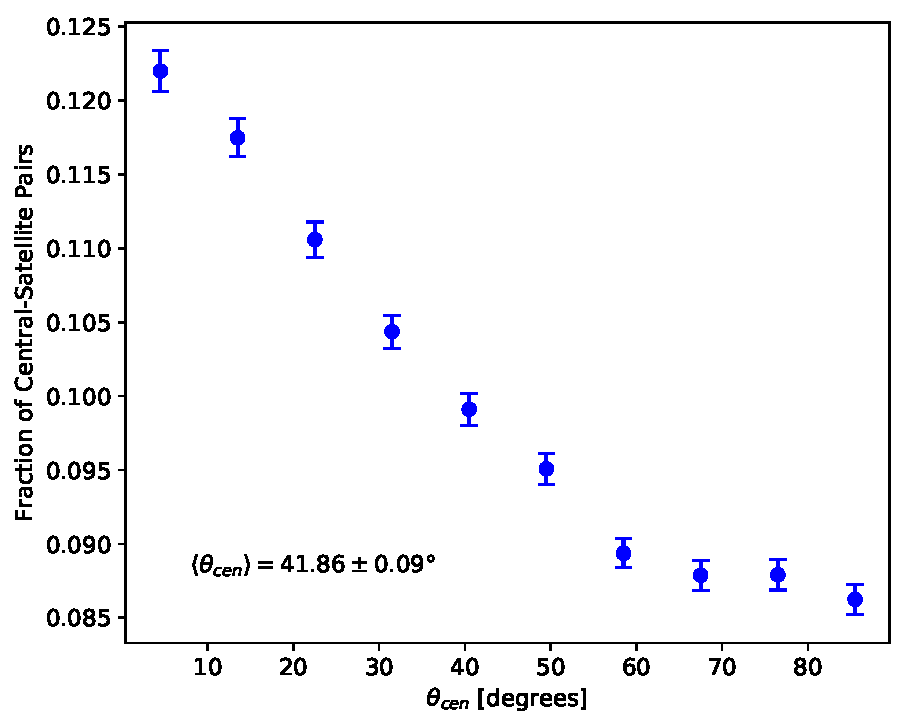
\includegraphics[width=\columnwidth]{theta_cen.pdf}
\end{center}
\caption[]{The distribution of the alignment of satellite galaxy positions relative to the position angle of the central galaxy of the cluster ($\theta_{\mathrm{cen}}$). There is a slight preference for satellite galaxies to be aligned closer to the major axis of the central galaxy.
\label{fig:thetacen}}
\end{figure}

\begin{figure}
\begin{center}
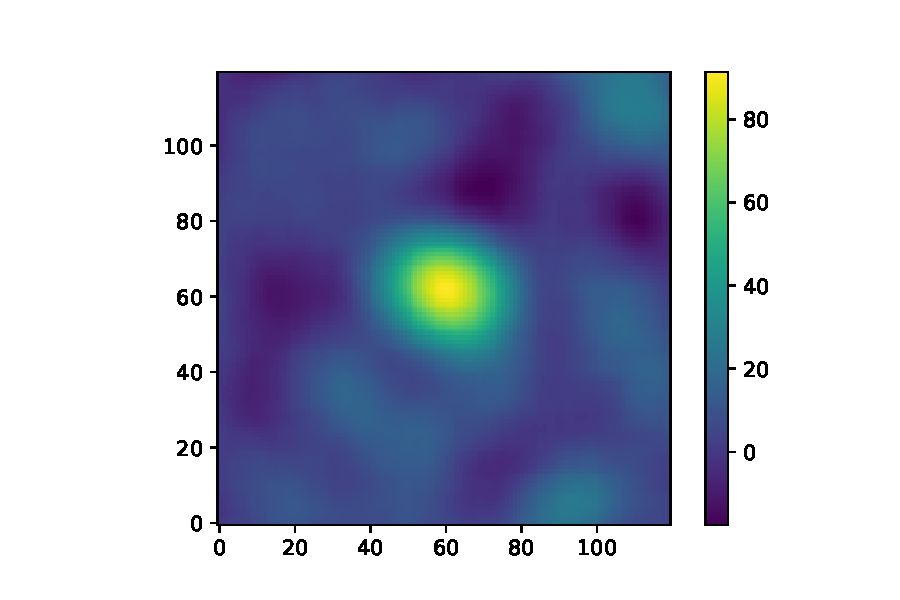
\includegraphics[width=\columnwidth]{massmap_2mom_norot.pdf}
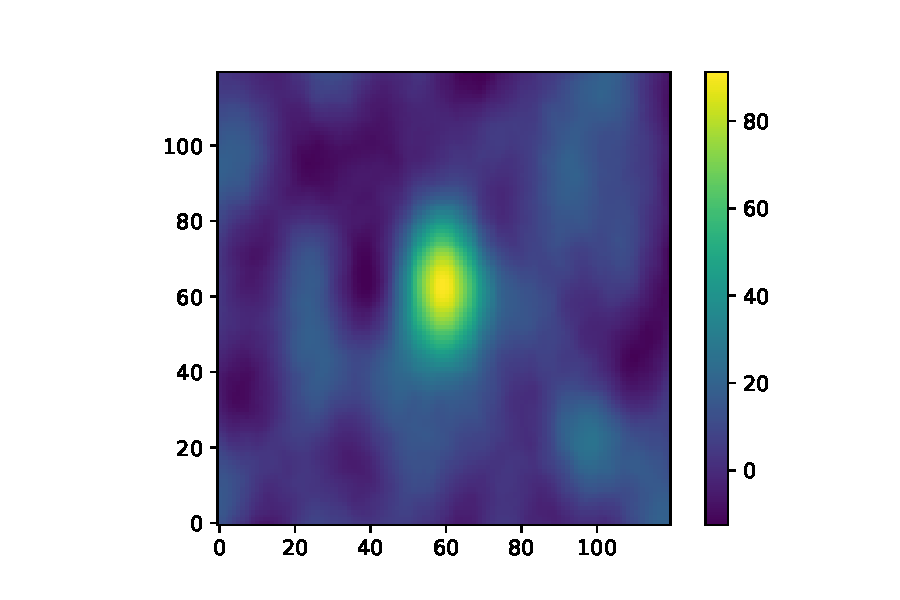
\includegraphics[width=\columnwidth]{massmap_2mom.pdf}
\end{center}
\caption[]{The stacked convergence map centered on the positions of clusters. \emph{Top}: The stacked convergence for clusters with their original orientation on the sky. \emph{Bottom}: The stacked convergence for clusters rotated with the position angle inferred from the satellite galaxy distribution oriented vertically. 
\label{fig:mass}}
\end{figure}

\subsection{Agreement between halo orientation and galaxy distribution}

We have used the distribution of satellite galaxies within clusters as a proxy for the shape of the underlying dark matter halo, which is what would drive any true intrinsic alignment of the galaxies. To justify this, we compare our cluster shape measurements inferred from the galaxy distribution with the DES Y1 weak lensing convergence `mass' map to confirm the correlation between galaxy satellite distribution and the underlying dark matter halo. The region around each cluster is cutout from the mass map, rotated, and stacked so that the inferred position angle from Sec. \ref{align1} is aligned for all clusters. We show this result in Fig. \ref{fig:mass}, which compares the stacked convergence with original random orientations, which has a nearly isotropic shape, with the cluster stack aligned by position angle, which has a highly anisotropic shape aligned in the direction of the inferred position angle of the stacked clusters. The ellipticity inferred from the stacked convergence is 0.326 \verify{...}, which agrees well with that inferred from the methods discussed in Sec. \ref{align1}, 0.348\verify{...}.

\begin{figure}
\begin{center}
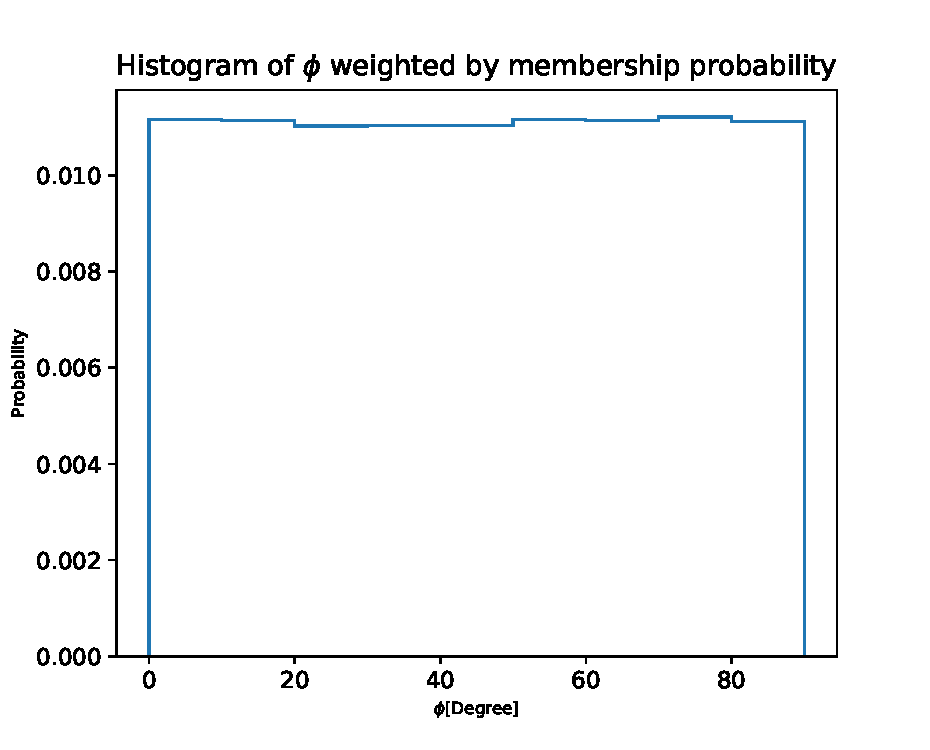
\includegraphics[width=\columnwidth]{phi_hist.pdf}
\end{center}
\caption[]{The distribution of angles $\phi_{\mathrm{sat}}$ between the position angle of each satellite galaxy and the line connecting it to the central galaxy of the cluster. The distribution is consistent with flat, with mean $\phi_{\mathrm{sat}}=44.9\pm 0.8$\textdegree, indicating no significant mean radial alignment among all satellite galaxies. 
\label{fig:phisat}}
\end{figure}

% \begin{figure}
% \begin{center}
% 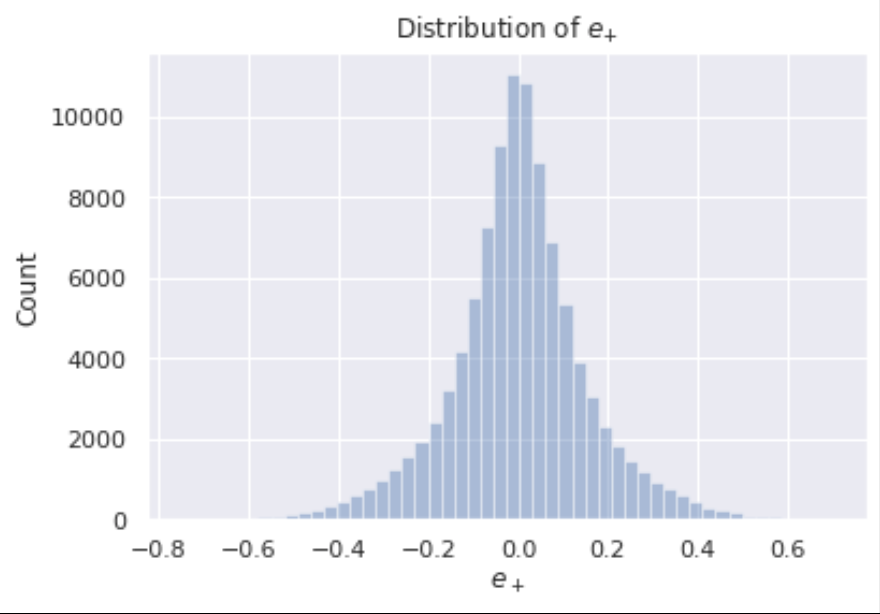
\includegraphics[width=\columnwidth]{eplus.png}
% 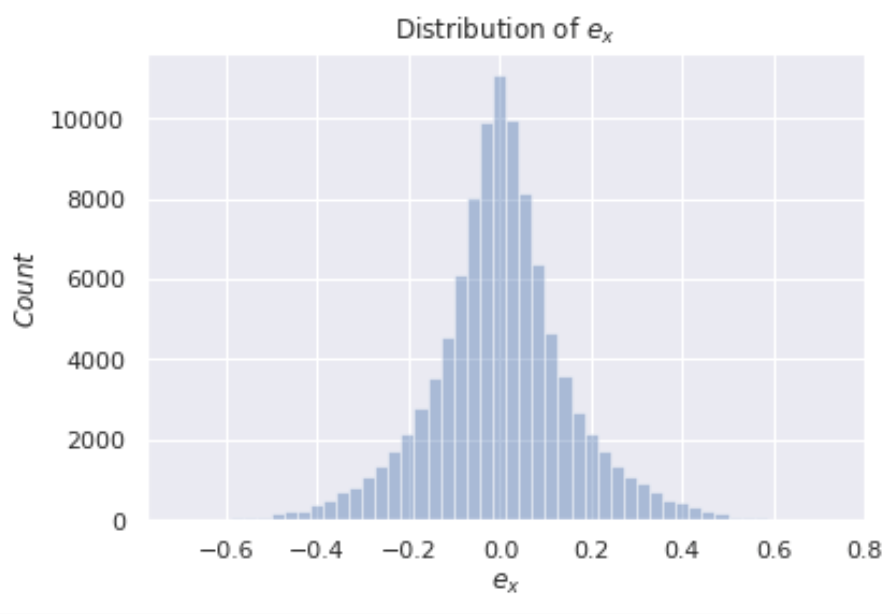
\includegraphics[width=\columnwidth]{ecross.png}
% \end{center}
% \caption[]{
% \label{fig:epc}}
% \end{figure}


\begin{figure}
\begin{center}
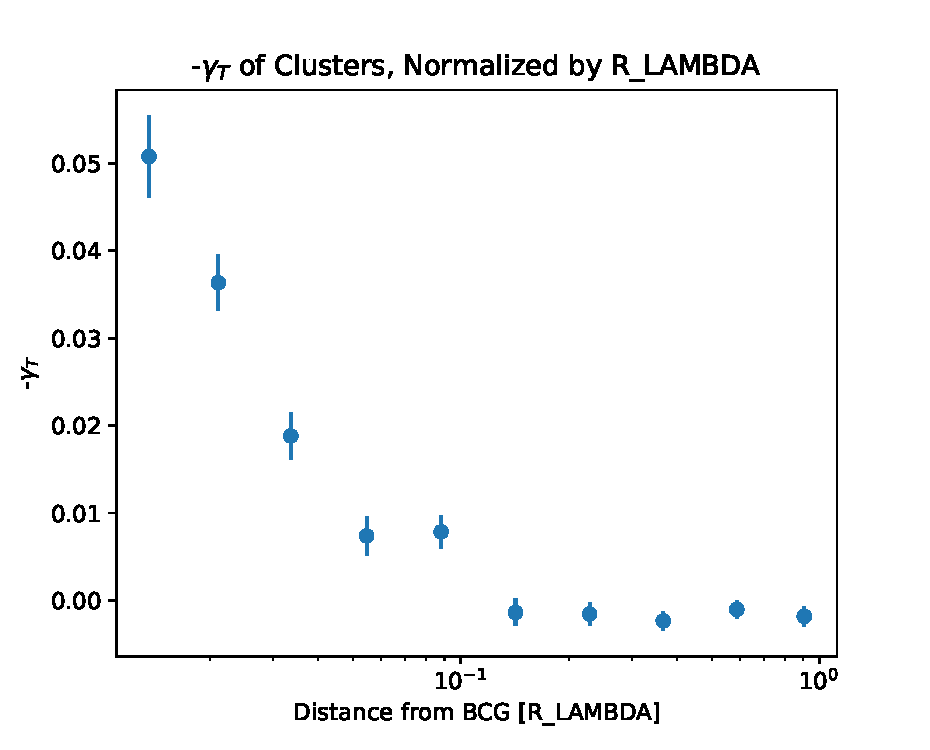
\includegraphics[width=\columnwidth]{gamma_T_rel.pdf}
\end{center}
\caption[]{The two-point correlation function $\gamma_r$, measuring the mean radial shape as a function of satellite distance from the center of the cluster. Within 0.1$R_\lambda$, there is a very significant radial intrinsic alignment signal, which is consistent with zero on larger scales.
\label{fig:gammar}}
\end{figure}


\begin{figure}
\begin{center}
%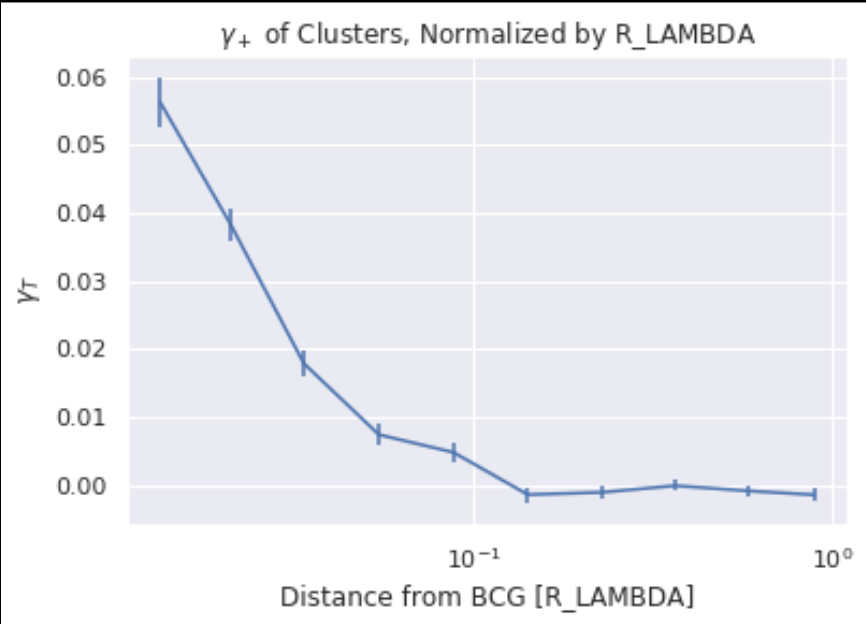
\includegraphics[width=\columnwidth]{gammar.png}
\end{center}
\caption[]{Several tests of potential systematic contributions to the measured $\gamma_r$ in Fig. \ref{fig:gammar}. 1) The cross-component $\gamma_x$. 2) The $\gamma_r$ signal measured using foreground galaxies around cluster centers. 3) The $\gamma_r$ signal measured using background galaxies around cluster centers. Tests (1) \& (2) are expected to be consistent with zero, while (3) should show a tangential shear signal due to gravitational lensing. These are confirmed by the measurements.
\label{fig:gammax}}
\end{figure}



\subsection{Radial alignment of satellite galaxies}\label{radial}

In addition to the alignment of the central galaxy with the dark matter halo of the cluster, satellite galaxies may also be influenced by the local tidal field, causing a radial alignment of their major axes. We show the distribution of $\phi_{\mathrm{sat}}$, the relative angle of the satellite major axis relative to the line connecting it to the central galaxy of the cluster, in Fig. \ref{fig:phisat}. We find no evidence for a non-flat distribution, with mean $\phi_{\mathrm{sat}}=44.9\pm 0.8$\textdegree, indicating no statistically significant mean radial alignment of objects within the cluster.

We also measure the mean radial shape as a function of distance from the cluster center $\gamma_r(R)$, which is shown in Fig. \ref{fig:gammar}, with distance from the center of the cluster as a fraction of the cluster size. We find a a highly significant radial alignment signal within about $0.1 R_{\lambda}$ of the cluster centers, with a total signal-to-noise $S/N=18$, where $(S/N)^2=\gamma_r^{\mathrm{T}} C^{-1} \gamma_r$. This signal is substantially stronger in amplitude and signal-to-noise than found with SDSS redMaPPer clusters in \cite{Huang_2016}.

To test the robustness of this measurement, we repeat it for a sample of galaxies not physically associated with the cluster, but projected in the same line of sight behind and in front of the cluster, finding a tangential shear and null signal, respectively. We also show the result of the $\gamma_x(R)$ cross-component measurement, which is also consistent with zero. These are shown in Fig. \ref{fig:gammax}.

Given the signal-to-noise of the measurement, we can attempt to look for evolution of the signal, for example in redshift or absolute magnitude in the . Given recent potential richness-dependent systematics, we also consider the richness-dependent. These results are shown in Fig. \ref{fig:gammar2}. \verify{summarize final results}

\subsection{Impact of radial alignment within clusters on cosmology}

Given the presence of such a significant radial alignment signal within redMaPPer clusters, it is necessary to consider if this signal could leak into estimates of mean tangential shear like $\gamma_t$ or $\Delta\Sigma$. In the cluster lensing measurements in \cite{}, a buffer in source photometric redshift of 0.1 was used to remove any sources within $z=0.1$ of the cluster to minimize these effects, but due to the uncertainty in source redshifts, this leaves a substantial fraction of cluster members as part of the source catalog. To test any impact of radial alignment leakage, we explicitly remove all cluster members from the source catalog and repeat the measurements in the same bins of richness and redshift. We find no change in the measured the lensing signal.

\begin{figure}
\begin{center}
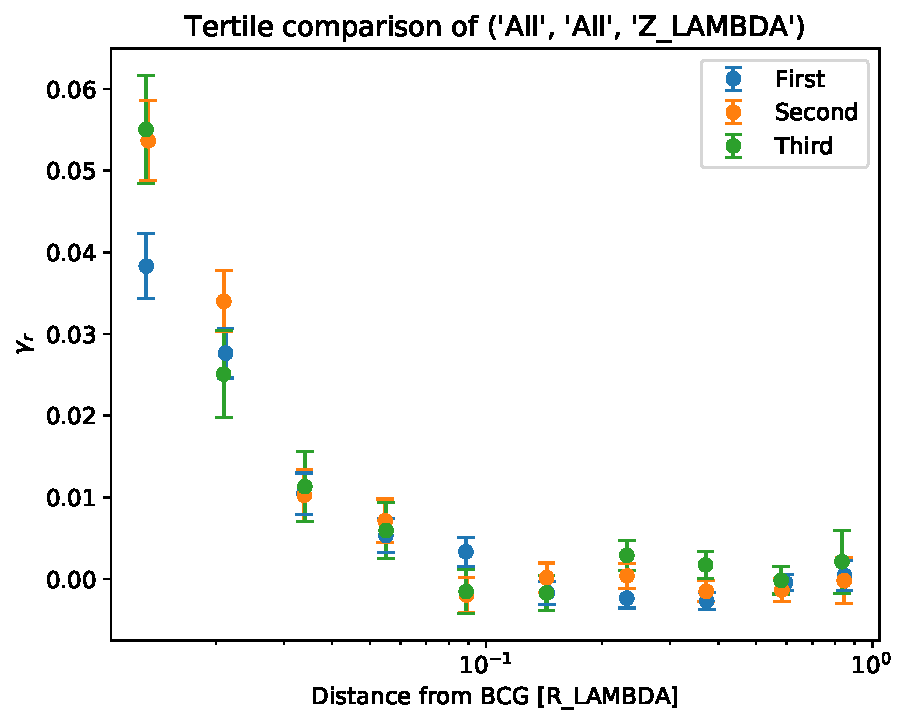
\includegraphics[width=\columnwidth]{zhou_z_tertile.pdf}
\end{center}
\caption[]{$\gamma_r$ measured for satellite galaxies split into bins of redshift, richness, and absolute magnitude. \verify{...}
\label{fig:gammar2}}
\end{figure}

\begin{figure}
\begin{center}
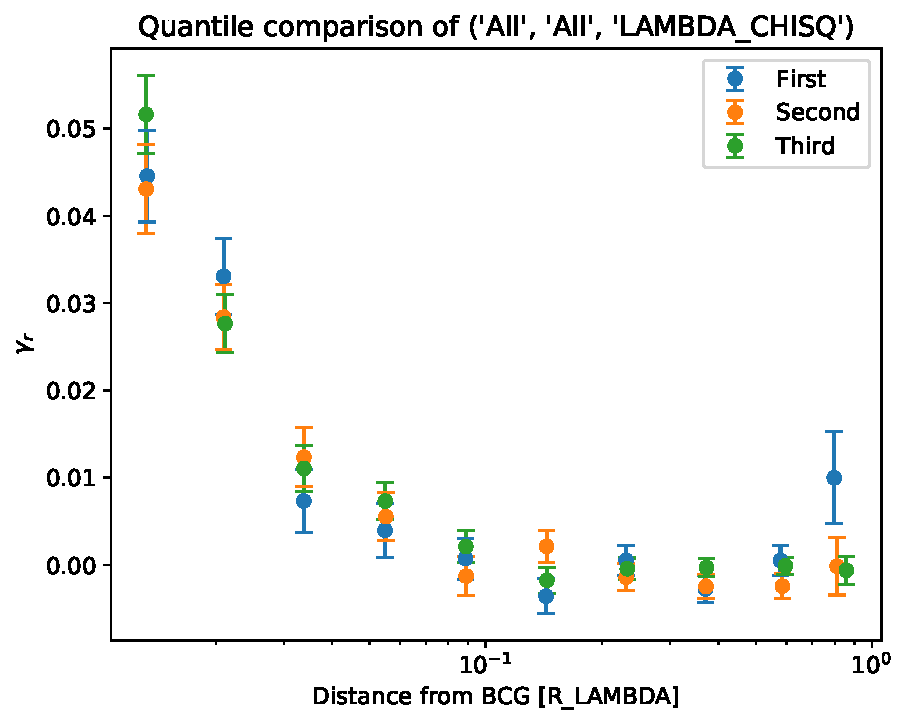
\includegraphics[width=\columnwidth]{zhou_lambda_tertile.pdf}
\end{center}
\caption[]{$\gamma_r$ measured for satellite galaxies split into bins of redshift, richness, and absolute magnitude. \verify{...}
\label{fig:gammar2}}
\end{figure}

\section{Conclusions}



\section*{Acknowledgements}

MT is supported by ... 

Funding for the DES Projects has been provided by the U.S. Department of Energy, the U.S. National Science Foundation, the Ministry of Science and Education of Spain, 
the Science and Technology Facilities Council of the United Kingdom, the Higher Education Funding Council for England, the National Center for Supercomputing 
Applications at the University of Illinois at Urbana-Champaign, the Kavli Institute of Cosmological Physics at the University of Chicago, 
the Center for Cosmology and Astro-Particle Physics at the Ohio State University,
the Mitchell Institute for Fundamental Physics and Astronomy at Texas A\&M University, Financiadora de Estudos e Projetos, 
Funda{\c c}{\~a}o Carlos Chagas Filho de Amparo {\`a} Pesquisa do Estado do Rio de Janeiro, Conselho Nacional de Desenvolvimento Cient{\'i}fico e Tecnol{\'o}gico and 
the Minist{\'e}rio da Ci{\^e}ncia, Tecnologia e Inova{\c c}{\~a}o, the Deutsche Forschungsgemeinschaft and the Collaborating Institutions in the Dark Energy Survey. 

The Collaborating Institutions are Argonne National Laboratory, the University of California at Santa Cruz, the University of Cambridge, Centro de Investigaciones Energ{\'e}ticas, 
Medioambientales y Tecnol{\'o}gicas-Madrid, the University of Chicago, University College London, the DES-Brazil Consortium, the University of Edinburgh, 
the Eidgen{\"o}ssische Technische Hochschule (ETH) Z{\"u}rich, 
Fermi National Accelerator Laboratory, the University of Illinois at Urbana-Champaign, the Institut de Ci{\`e}ncies de l'Espai (IEEC/CSIC), 
the Institut de F{\'i}sica d'Altes Energies, Lawrence Berkeley National Laboratory, the Ludwig-Maximilians Universit{\"a}t M{\"u}nchen and the associated Excellence Cluster Universe, 
the University of Michigan, NFS's NOIRLab, the University of Nottingham, The Ohio State University, the University of Pennsylvania, the University of Portsmouth, 
SLAC National Accelerator Laboratory, Stanford University, the University of Sussex, Texas A\&M University, and the OzDES Membership Consortium.

Based in part on observations at Cerro Tololo Inter-American Observatory at NSF’s NOIRLab (NOIRLab Prop. ID 2012B-0001; PI: J. Frieman), which is managed by the Association of Universities for Research in Astronomy (AURA) under a cooperative agreement with the National Science Foundation.

The DES data management system is supported by the National Science Foundation under Grant Numbers AST-1138766 and AST-1536171.
The DES participants from Spanish institutions are partially supported by MICINN under grants ESP2017-89838, PGC2018-094773, PGC2018-102021, SEV-2016-0588, SEV-2016-0597, and MDM-2015-0509, some of which include ERDF funds from the European Union. IFAE is partially funded by the CERCA program of the Generalitat de Catalunya.
Research leading to these results has received funding from the European Research
Council under the European Union's Seventh Framework Program (FP7/2007-2013) including ERC grant agreements 240672, 291329, and 306478.
We  acknowledge support from the Brazilian Instituto Nacional de Ci\^encia
e Tecnologia (INCT) e-Universe (CNPq grant 465376/2014-2).

This manuscript has been authored by Fermi Research Alliance, LLC under Contract No. DE-AC02-07CH11359 with the U.S. Department of Energy, Office of Science, Office of High Energy Physics.

%%%%%%%%%%%%%%%%%%%%%%%%%%%%%%%%%%%%%%%%%%%%%%%%%%

%%%%%%%%%%%%%%%%%%%% REFERENCES %%%%%%%%%%%%%%%%%%

% The best way to enter references is to use BibTeX:

\bibliographystyle{mnras}
\bibliography{short} % if your bibtex file is called example.bib


%%%%%%%%%%%%%%%%%%%%%%%%%%%%%%%%%%%%%%%%%%%%%%%%%%

%%%%%%%%%%%%%%%%% APPENDICES %%%%%%%%%%%%%%%%%%%%%

\appendix

\section{Some extra material}

If you want to present additional material which would interrupt the flow of the main paper,
it can be placed in an Appendix which appears after the list of references.

%%%%%%%%%%%%%%%%%%%%%%%%%%%%%%%%%%%%%%%%%%%%%%%%%%


% Don't change these lines
\bsp	% typesetting comment
\label{lastpage}
\end{document}

% End of mnras_template.tex